%\documentclass[12pt]{amsart}
\documentclass[12pt, letterpaper]{article}
%\usepackage{geometry}                % See geometry.pdf to learn the layout options. There are lots.
%\geometry{letterpaper}                   % ... or a4paper or a5paper or ... 
%\geometry{landscape}                % Activate for for rotated page geometry
%\usepackage[parfill]{parskip}    % Activate to begin paragraphs with an empty line rather than an indent
\usepackage{graphicx}
\usepackage{amssymb}
\usepackage{epstopdf}
\DeclareGraphicsRule{.tif}{png}{.png}{`convert #1 `dirname #1`/`basename #1 .tif`.png}

\usepackage[top=1.1in, bottom=1.1in, left=1.4in, right=1.4in]{geometry}
\usepackage{natbib}
\usepackage{amssymb}
%\usepackage{natbib}
\usepackage{color}
\usepackage{graphicx}
\usepackage{fancyhdr}
\usepackage[T1]{fontenc}
\usepackage{titling}
\usepackage{sectsty}
\usepackage{sidecap}
\usepackage{placeins}
\usepackage{indentfirst}
\usepackage{wrapfig}


\usepackage{setspace}  % Needed for Double Spacing
\usepackage[english]{babel}
\usepackage{lipsum}

\pagestyle{fancy}
\lhead{Dr. Ana-Maria A. Piso}
\rhead{NPP Research Proposal}

\DeclareGraphicsRule{.tif}{png}{.png}{`convert #1 `dirname #1`/`basename #1 .tif`.png}

\title{THE ROLE OF DISK VOLATILE CHEMISTRY AND DYNAMICS IN SHAPING THE COMPOSITIONS OF NASCENT PLANETS}  % add title here
\author{DR. ANA-MARIA A. PISO}  % include Author's name here
%\date{}                                           % Activate to display a given date or no date

\begin{document}
\maketitle

\doublespacing

\noindent
\textbf{Title of Research Opportunity}: STAR AND PLANET FORMATION (18361)\\
\smallskip
\noindent
\textbf{NASA Center}: JET PROPULSION LABORATORY\\
\smallskip
\noindent
\textbf{NASA Advisor}: DR. NEAL TURNER \\
\smallskip


\begin{abstract}

%Type your Abstract here. The abstract should be a brief summary of the scientific problem to be addressed, your proposed research strategy, your methodology, and expected results.

The compositions of giant planets are determined by and tightly connected to the composition of the protoplanetary disk in which they are born. In turn, disks are affected by a multitude of chemical and dynamical processes that affect their composition both spatially and temporally. While the evolution and chemical composition of disks and gas giant atmospheres have been explored separately from the dynamical or chemical perspective, studies that investigate the coupled effect of chemistry and dynamics on the disk and planet evolution do not exist to date. I will develop a self-consistent chemo-dynamical model to explore how the disk dynamics and chemistry, as well as the dynamics of planetesimals and planetary embryos, affect the compositions of mature giant planets that we see today. Through analytical and numerical calculations, I will investigate a range of chemical and dynamical processes that may affect a disk's, and hence a planet's, composition at different locations in the disk midplane. I will then generalize the above results by inputting them into a large planet synthesis model, in which I will explore a wide range of initial disk and planetary embryo conditions. This will enable me to (1) predict the kinds of giant planet compositions that can be obtained from planet formation at different disk locations, and (2) back-track a planet's formation location based on its composition. 
\end{abstract}

\section{STATEMENT OF PROBLEM}

%State the scientific problem you plan to address.  Put the problem in context and discuss the importance of the problem and its relevance to NASA?s goals and missions specifically, and its relevance to the field in general.

Within the last two decades, more than one thousand extrasolar planets (exoplanets) have been discovered $[1]$. Their diversity in terms of mass, radius, location and composition $[2]$ provides an exciting field of research, with the eventual goal of finding planets that are similar to our own Earth and may sustain life. For this purpose, it is thus crucial to explore and understand how planets obtain their compositions. Observations of Earth-like planets that can provide useful insight about their composition are challenging --- the solid interior structure of terrestrial planets cannot be detected, and their gaseous envelopes are small by comparison (both in mass and radius), which makes it difficult to obtain atmospheric spectra and find out what chemical compounds they are made of. We therefore turn to giant planets, which have provided a rich and intriguing research area for decades. Gas giants contain most of their mass in their atmosphere, hence their chemical composition is determined by that of their envelopes. The last few years have seen a substantial increase in the number of giant planets with observed atmospheric spectra (e.g., $[3]$, $[4]$), which has enhanced our understanding of these planets' chemical structure, and has provided us with quantitative information about the abundances of various compounds in their envelopes besides hydrogen and helium. Finally, gas giants shape the architecture of planetary systems and affect the delivery of volatile compounds to terrestrial planets, which has direct consequences for the habitability of worlds similar to our own. Thus testing theories of planet formation against gas giant compositions will help constrain planet formation theories more generally.     

Both terrestrial and giant planets are born in protoplanetary disks, which implies that their \textbf{compositions are determined by and tightly linked to the structure and composition of the disk}. The chemical and dynamical evolution of disks, as well the formation of giant planets have both been previously investigated in isolation. However, the coupled chemo-dynamical disk evolution, planet compositions, and most importantly the disk-planet connection have not yet been considered in detail. As shown in my work on the minimum core mass of gas giants ($[5]$, $[6]$), planet formation depends sensitively on disk physics and chemistry. \textbf{I propose to develop a holistic chemo-dynamical framework to explore how disk dynamics and chemistry, as well as the dynamics of nascent planets and planetesimals, regulate the compositions of mature giant planets.} Such a model will enhance our understanding of planetary structures by enabling us to \textbf{predict what kind of planet compositions result from planet formation in different parts of the disk}, as well as \textbf{constrain a planet's formation location based on its chemical composition}. %Furthermore, this work provides essential context for characterizing the gas giants that instruments such as the James Webb Space Telescope (JWST) and the Transiting Exoplanet Survey Satellite (TESS) will one day discover. %\textbf{My proposed work has therefore direct relevance to NASA's Exoplanet Exploration Program.}

\subsection*{Relevance to NASA's Missions}

The research outlined above is directly related to NASA's Exoplanet Exploration Program. Applying my proposed theoretical framework to a wide range of disk and planetary embryos initial conditions will provide essential context for characterizing the atmospheric compositions of gas giants that instruments such as the \textbf{James Webb Space Telescope (JWST)} and the \textbf{Wide Field Infrared Survey Telescope (WFIRST)} will discover in the near future. Moreover, my results will be useful in selecting the most promising giant planets, from a compositional point of view, for eventual follow-up with JWST. With my current theoretical expertise and the skills that I will gain as a NASA Postdoctoral Fellow, I am in the position of playing a leading role in interpreting the compositions of newfound giant planets, and in using planet compositions as tracers of planet formation locations. 


\section{SCIENCE BACKGROUND}

%Discuss the background of the problem that you propose to address.  Review the history of the problem, discuss progress in this field, and discuss what is needed to further advance the field.  Include citations and references as necessary (you should use an accepted citation format relevant for your field).

The chemical composition of protoplanetary disks is largely determined by the freeze-out of volatile species. The snowline locations of volatile molecules are thus crucial in determining the chemical abundances in gas and dust throughout the disk, as well as planet compositions. 

One important effect of the existence of snowlines is that disks are expected to contain different amounts of volatiles in gas and in dust at different locations. As the main carbon and oxygen carriers, i.e. H$_2$O, CO$_2$ and CO, are amongst the most abundant volatiles in comets and protostellar cores ([7], [8], [9]), variations in the carbon-to-oxygen (C/O) ratio in gas and dust throughout a disk are particularly important. This issue was first addressed by [10]. Figure \ref{fig:oberg} shows the C/O ratio in gas and dust as a function of semimajor axis, assuming protostellar abundances for the volatiles. The C/O ratio in gas is enhanced compared to the stellar value, particularly between the CO$_2$ and CO snowlines where it reaches unity. 

\begin{figure}[h!]
\centering
\includegraphics[width=0.7\textwidth]{oberg11.png}
%\vspace{-0.5in}
\caption{The C/O ratio in gas (solid line) and dust (dashed line) as a function of semimajor axis in a static disk. The dotted line shows the stellar value of 0.54. Gas-phase C/O ratios of order unity can be achieved in the outer disk. From [10]. }
\label{fig:oberg}
\end{figure}

The pioneering work of [10], as well as the purported detection of a superstellar gas-phase C/O ratio in the atmosphere of WASP 12-b [11], inspired further theoretical investigations into the C/O ratio in disk and planet atmospheres. The model of [11] assumes a static disk, thus ignoring disk chemistry or dynamics. In reality, however, there are many chemical and dynamical processes that occur in disks (see [9] for a review), which will change the chemical molecular and elemental abundances, and therefore C/O ratios. For example, [12] calculate the C/O ratio throughout the disk including dynamical effects such as radial drift, grain coagulation, and the diffusion of volatile vapors. [13] include planetary migration in their C/O ratio calculation, and use the C/O ratio to constrain migration mechanisms. Additional carbon volatile carriers, such as CH$_4$, are considered by [14],  and they find that the gas-phase C/O ratio may be enriched by up to a factor of four compared to the Solar value in the outer disk.  While the C/O ratio is an important signature of disk and planet atmospheric chemistry, many other compounds have been detected in disks [9], which may affect the composition of disks and of nascent planets even when only dynamical processes are included and the chemistry is static, such as in the studies described above. 

From the chemistry perspective, several studies have modeled the chemical evolution of disk volatile abundances using chemical networks with hundreds to thousands of reactions (see., e.g., [15], [16] and references in [9]); however, most of these works do not consider any dynamical processes.   

In my recent work ([17], [18]), I explored the effect of radial drift of solids and viscous gas accretion onto the central star, as well as different ice compositions, on snowline locations and the C/N/O ratios in disks. Besides C and O carriers, I also considered nitrogen-bearing species, such as N$_2$ and NH$_3$. Figure \ref{fig:CO_ratio} shows that the processes described above can change the location of the CO snowline by up to a factor of $\sim$7, thus introducing a large uncertainty in the position of the CO snowline, and therefore the disk locations where the gas-phase C/O ratio is enhanced compared to the stellar value. The same effect was observed for the N$_2$ snowline location.

\begin{figure}[h!]
\centering
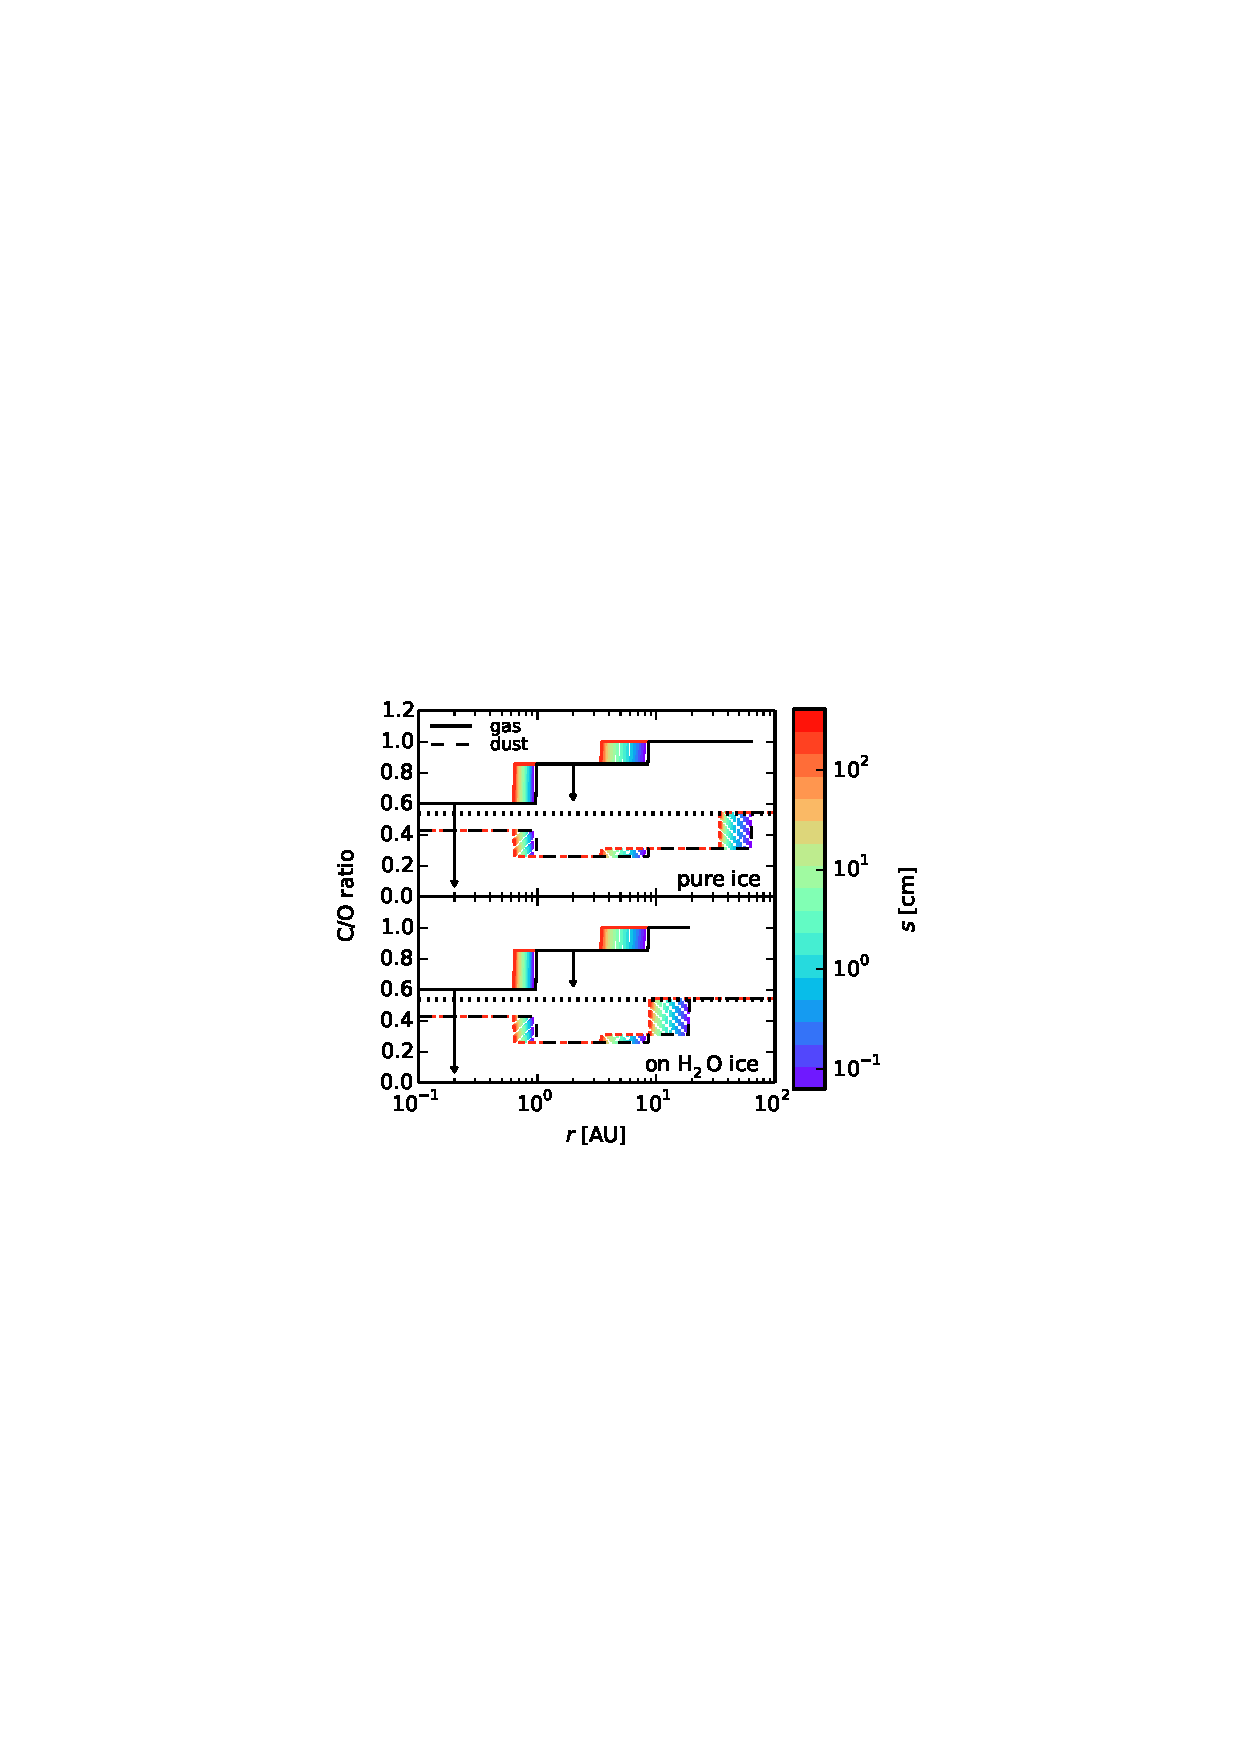
\includegraphics[width=0.8\textwidth]{C_O_water_ice.pdf}
%\vspace{-0.5in}
\caption{C/O ratio estimates in gas (solid lines) and dust (dashed lines) as function of semimajor axis in a viscous disk, for CO as pure ice (top panel) or as water dominated ices (bottom panel). The H$_2$O, CO$_2$ and CO snowlines are shown for particles with initial sizes $\sim0.05$ cm $\lesssim s \lesssim$ 7 m as indicated by the color bar. The C/O ratio in a static disk (black lines) is shown for comparison. Taken together, disk dynamics and ice compositions move the CO snowline inward by a factor of $\sim$7. From [17].} 
\label{fig:CO_ratio}
\end{figure}

It it thus clear that, in order to better understand and constrain disk and planet compositions, as well as use planet compositions as tracers of planet formation locations, the following are necessary: (1) the consideration of additional dynamical effects, (2) a self-consistent coupling of disk chemistry and dynamics, (3) the inclusion of planet dynamical effects in order to explore the disk-planet connection, and (4) applying (1), (2) and (3) to a wide parameter space of disk and planetary embryos initial conditions.   


\section{GENERAL METHODOLOGY}

%Discuss the strategies and methods you will use. Describe why you chose your particular plan, and discuss how this plan improves upon previous work in this field.

\subsection{Coupled Chemical and Dynamical Disk Evolution} 
%\underline{\textbf{1. Coupled Chemical and Dynamical Disk Evolution}}

Protoplanetary disks experience a multitude of chemical and dynamical processes, as shown schematically in Figure \ref{fig:disk}. These processes affect the disk structure and composition, and thus the composition of nascent planets. As shown in Figure \ref{fig:chemical}, the timescales for various disk chemical and dynamical processes may be comparable at least in some parts of the disk. It follows that these two effects cannot be decoupled, and that the chemo-dynamical evolution of the disk has to be studied simultaneously and self-consistently. Through \textbf{analytical and numerical calculations}, I will first explore a \textbf{range of dynamical processes that may affect the distribution of volatiles in disks}, expanding and generalizing the framework I developed during my dissertation research ($[17]$, [18]). Such effects include particle growth and fragmentation, as well as accretion rate and stellar luminosity evolution.   

\begin{figure}[h!]
\centering
\includegraphics[width=\textwidth]{disk}
\vspace{-0.1in}
\caption{Sketch of chemical and dynamical processes in a protoplanetary disk around a Sun-like star (from $[9]$).}
\label{fig:disk}
\end{figure}



From the chemistry perspective, molecular abundances vary significantly across a typical disk, due to steep gradients in temperature, density and radiation. 
%Figure 1 shows a theoretical example of how both changes in disk temperature, as well as time evolution, decrease the abundance of carbon monoxide (CO) by several orders of magnitude \cite{aikawa96}. 
The complexity of disk chemistry means that coupling it with dynamical processes, while necessary, is non-trivial.  I will couple the dynamical framework outlined above with \textbf{time-dependent chemical models of increasing complexity}, informed by results from state-of-the-art disk chemistry models (that can only be run on static disks). This will show how the snowline locations of volatiles, as well as the chemical composition of the disk gas and dust evolve, which has \textbf{direct implications on the compositions of young planets}. Moreover, since I am primarily interested in processes that affect the disk mid-plane where planets form, my results could be simplified by the fact that certain chemical processes may not be important in this disk parameter space.

\begin{figure}[h!]
\centering
\includegraphics[width=\textwidth]{chemical_timescales}
\vspace{-0.3in}
\caption{The distribution of characteristic chemical and dynamical timescales $\tau$ in disks as a function of semi-major axis and height. The numbered curves are $\log_{10} (\tau)$ in years (from $[28]$).}
\label{fig:chemical}
\end{figure}

\textbf{My results from this step will be useful in interpreting JWST observations of volatile abundances and ratios in protoplanetary disk atmospheres.} The JWST \textbf{Mid-Infrared Instrument (MIRI)} (see, e.g., [19] for an overview) will enable abundance measurements of species such as H$_2$O, CO$_2$, C$_2$H$_2$, HCN in the atmospheres of a much broader range of disks that it was possible with the Spitzer Space Telescope (e.g., [20]). \textbf{Varying disk initial conditions, such as the temperature profile and initial species abundances}, and comparing them with the known properties of disks that JWST will observe, will help me in explaining \textbf{volatile ratios from the JWST data.} This step should be completed within 8 months.



%this dynamical model  develop a (chemical models of increasing complexity) simplified time-dependent chemistry, 


%\vspace{0.2in}
\subsection{Planet and Planetesimal Migration}
%\underline{\textbf{2. Planet and Planetesimal Migration}}

The complex processes outlined in part 1 will directly impact the composition and dynamics of forming gas giants, as the latter are born and evolve simultaneously with the disk. 
\begin{figure}[h!]
\centering
\includegraphics[width=0.5\textwidth]{HLTau_nrao}
%\vspace{-0.5in}
\caption{ALMA continuum image of the disk around HL Tau, which shows evidence of a gas gap in the disk, most likely created due to planetary migration (from $[26]$).}
\label{fig:HLtau}
\end{figure}
The chemical evolution of the gas disk molecular abundances, as well as disk dynamics, determine how a young planet's atmospheric composition changes in time and with the planet's location, and therefore the final chemical structure of mature planets. \textbf{It is thus clear that disks and planets are deeply connected, and that this relation needs to be explored}. %I will add planetary embryos in the code developed in step 1, and 

Giant planets can migrate through the disk while still accumulating gas. Figure \ref{fig:HLtau} shows an exciting ALMA observation of a planetary gap in the disk around HL Tau $[26]$. This will change a planet's atmospheric composition since the disk chemical abundances are different at different disk locations. Additionally, giant planets may still accumulate planetesimals while accreting nebular gas $[10]$. The final composition of a planet's atmosphere will thus depend on how much gas and solids are accreted in this stage. \textbf{I will add planet dynamical effects such as migration and planetesimal accretion in the chemical and dynamical model developed in part 1, and quantify how these processes affect the chemical composition of gas giant envelopes}. This step should be completed within 8 months.


%\vspace{0.2in}

\subsection{Model Planet Populations} 
%\underline{\textbf{3. Model Planet Populations}}

The results from parts 3.1 and 3.2 will feed into a \textbf{large planet synthesis model}, in which I will use a grid of different \textbf{initial disk and planetary embryo conditions}. I will develop my own numerical program instead of using already existing codes of planet population synthesis (e.g., $[27]$ and references therein), since the latter involve many complex physical processes, some of which might not be necessary or relevant for my own calculations. To minimize computational expenses, I will build a program from bottom-up that includes select physical and chemical processes based on the local simulations from steps 1 and 2. 

Based on the framework that I developed during my dissertation ([5], [6]), I will use the \textbf{core accretion model} for the formation of gas giants. The growth rate of giant nascent planets before the dispersal of the protoplanetary disk is highly dependent on the opacity of their envelopes. However, disk and atmosphere opacities are highly uncertain. I will therefore explore \textbf{a range of opacity models appropriate for different disk regions and temperatures, considering both dusty and grain-free envelopes}. (e.g., [21], [22], [23]). Since I am interested in the chemical composition of both nascent and mature giant planets, \textbf{I will carry my planet synthesis model forward through the dispersal of the gas disk}. Physical processes to be considered in this evolutionary stage are, for example, \textbf{spontaneous mass loss} due to loss of pressure support from the disk [24], or \textbf{dynamical interactions with forming terrestrial planets.}  Through numerical calculations, I will expand the analytic model of [24] for atmospheric mass loss. This will enable me to obtain \textbf{robust quantitative results} for the physical properties of gas giants that we see today, as well as \textbf{explore a broader range of disk and planet parameter space}. The latter will be particularly relevant for connecting my predictions with JWST detections, which will observe giant planets with a variety of masses, semimajor axes, and compositions.    

To conclude, my proposed planet synthesis model will allow me to predict the \textbf{range of planet compositions that can form under reasonable disk conditions}, as well as \textbf{constrain a planet's formation location based on its chemical composition}. %Comparing my results with current observations of atmospheric spectra (e.g., Figure 3 from $[4]$), and more importantly future JWST observations, will lead to great scientific strides in understanding the complex connection between protoplanetary disks and the formation, evolution and composition of exoplanets. 
This step should be completed within 8 months.


\section{EXPLANATION OF NEW TECHNIQUES}

%Discuss in detail how your methods, plans and techniques are new or novel, and what advantages and disadvantages they have compared to previous work.

\subsection{Chemical Modeling}

Current state-of-the-art chemical networks include hundreds of molecules and reactions. The majority of these models, however, are not specifically focused on the disk mid-plane, which is the relevant parameter space for planet formation and thus for my goals. Moreover, as discussed in Section 3.1, some or many of the processes that these networks model may not penetrate all the way to the cold disk mid-plane. \textbf{I will select only the chemical processes that I deem suitable for the disk mid-plane, thus potentially greatly reducing the number of reactions and reactants}. This will result in \textbf{significantly lower computational times}. Furthermore, I will create a table of reactions and compounds relevant only for the disk mid-plane \textbf{and make it publicly available} as a useful tool for other astronomers interested in this chemical parameter space. 

\subsection{Disk Dynamical Processes} 

Most studies that explore the effect of disk dynamics on disk/planet compositions and the C/O ratio (e.g., [12], [14]) study the various dynamical effects they include in their respective models simultaneously. Thus the relative importance and impact of each dynamical process on their final results is often not clear. In contrast, \textbf{I will incorporate dynamical processes in my model gradually, and at each step quantify the effect of a given process}. This method will enable me to (1) \textbf{include only the dynamical processes that I find important in my planet synthesis model} (see Section 3.3), and (2) \textbf{more easily trace a planet's formation location based on its composition} after the simulation described in Section 3.3, \textbf{as I will know the importance of each dynamical effect} that will have led to a given planet composition. 

\subsection{Planet Synthesis Model}

As discussed in Section 3.3, I will build an \textbf{original and novel planet synthesis code}, which I will tailor to only include the chemical and dynamical processes that I find important for my science problem (see Sections 3.1., 3.2, 4.1., 4.2). In comparison with existing planet population synthesis programs, my model will have the advantage of \textbf{greatly decreasing computational costs}. Moreover, my complex chemo-dynamical planet synthesis model and code will serve as a useful \textbf{input of young model planets for subsequent atmospheric evolution codes}, such as is the case, for example, with the code developed by [25].  


\section{EXPECTED RESULTS}

%Discuss the results you expect to achieve and how these results will influence the development of the field of research regarding your science problem.

My expected results can be summarized as follows:

1. A clear understanding of the chemical processes and molecular compounds that are relevant in the disk mid-plane (i.e. the planet formation region), as well as the expected molecular and elemental abundances. This will be important for further theoretical work in this field, as well as for both predicting and interpreting current and future observations of gas giant atmospheric spectra.

2. Further insight into disk and planetary dynamical processes that affect the locations of volatile snowlines and the elemental ratios in disks and planet atmospheres. This, and the result outlined in point 1, will substantially improve our current understanding of how giant planets obtain their compositions. 

3. The results of my planet synthesis study will provide a robust framework of using a planet's composition as a tracer of its formation location. Furthermore, comparing my results with current observations of atmospheric spectra (e.g., Figure 3 from $[4]$), and more importantly future JWST observations, will lead to great scientific strides in understanding the complex connection between protoplanetary disks and the formation, evolution and composition of exoplanets. 


\begin{figure}[h!]
\centering
\vspace{-0.2in}
\includegraphics[width=\textwidth]{water_spectrum}
\vspace{-0.2in}
\caption{The transmission spectrum of exoplanet WASP-12b measured with the Hubble Space Telescope/Wide Field Camera 3. The white dots are the measured transit depths, the blue squares and dark blue line are the best fit model, while the shaded regions represent 1- and 2 $\sigma$ intervals in the retrieved spectrum. The increase in transit depth around $\sim$1.4 $\mu$m is evidence for a water feature in the atmosphere (from $[4]$).}
\label{fig:HLTau}
\end{figure}

%\textbf{MIT is the ideal place for me to pursue my postdoctoral work.} Its research facilities and academic excellence are unparalleled. I would love the opportunity to work with \textbf{Prof. Hilke Schlichting}, an expert in planet formation theory and dynamics --- such a collaboration would be instrumental in achieving my research goals during my postdoctoral tenure and afterwards. I would also like to collaborate with \textbf{Prof. Sara Seager}, a co-investigator of the TESS mission and a leading theorist in atmospheric chemistry, as well as with members of her group, who specialize in a broad range of exoplanet theory and computational topics. \textbf{Dr. Margaret Pan}, an excellent theorist in planetary dynamics and protoplanetary disks, will join the MIT EAPS department in early 2016 --- it would be a pleasure to work with her as well. Additionally, the MIT Physics department hosts leaders in detecting and characterizing worlds outside the Solar system, such as \textbf{Prof. Joshua Winn}, which presents great prospects in connecting my theoretical research work with observations. \\

%Finally, in order to connect my theoretical work with observations, I would like to collaborate with \textbf{Prof. Joshua Winn}, who is an expert in discovering and characterizing exoplanets. \\

%\textbf{The University of Chicago is the ideal place for me to pursue my postdoctoral research}, due to its vibrant community of experts in protoplanetary disks and exoplanets, both in the Department of Astronomy and Department of Geophysical Sciences. I would love the opportunity to work with \textbf{Prof. Leslie Rogers}, an expert in planetary interiors and atmospheres --- such a collaboration would be instrumental in achieving my research goals during my postdoctoral tenure and afterwards. In the Department of Geophysical Sciences, I would like to collaborate with \textbf{Prof. Fred Ciesla}, a leader in protoplanetary disk dynamics, chemical composition and evolution. Additionally, the Department of Astronomy hosts experts in detecting and characterizing worlds outside the Solar system, such as \textbf{Prof. Dan Fabrycky} and \textbf{Prof. Jacob Bean}, which presents great prospects in connecting my theoretical research work with observations. \\

%\textbf{Fred Ciesla} (proposed faculty host) is an expert in protoplanetary disk dynamics, as well as chemical composition and evolution. Leslie Rogers, who will begin her faculty appointment in Fall 2016, is a leader in exoplanet theory, specifically planetary interiors and atmospheres, so I would love the opportunity to collaborate with her on my postdoctoral work. Additionally, the University of Chicago Department of Astronomy hosts leaders in detecting and characterizing worlds outside the Solar system, such as Dan Fabrycky and Jacob Bean, which presents great prospects in connecting my theoretical research work with observations.

%\begin{figure}[h!]
%\centering
%\includegraphics[width=0.7\textwidth]{CO_abundances}
%%\vspace{-0.5in}
%\caption{TBD}
%\label{fig:CO}
%\end{figure}



%\if\bibinc n
%\bibliography{refs}
%\fi
\FloatBarrier
%\def\bibfont{\footnotesize}
%\setlength{\bibsep}{0.0pt}

%\section*{References}
\section{REFERENCES}
\singlespacing
%\begin{thebibliography} {9}
\noindent $[1]$ Batalha, N. M. 2014, Proceedings of the National Academy of Science, 111, 12647 \\
$[2]$ Lissauer J. J., Dawson R. I., \&Tremaine S., 2014, Nature, 513, 336 \\
$[3]$ Debes, J. H., Jang-Condell, H., Weinberger, A. J., Roberge, A., \& Schneider, G. 2013, ApJ, 771, 45 \\
$[4]$ Kreidberg, L., Line, M. R., Bean, J. L., et al. 2015, ApJ, 814, 66 \\
\textbf{$[5]$ Piso, A.-M. A., \& Youdin, A. N. Y. 2014, ApJ, 786, 21} \\
\textbf{$[6]$ Piso, A.-M. A., Youdin, A. N. Y., \& Murray-Clay, R. A. 2015, ApJ, 800, 82} \\
$[7]$ Rodgers, S. D., \& Charnley, S. B. 2002, MNRAS, 330, 660 \\
$[8]$ Mumma, M. J., \& Charnley, S. B. 2011, ARA\&A, 49, 471 \\
$[9]$ Henning, T., \& Semenov, D. 2013, Chemical Reviews, 113, 9016 \\
$[10]$ \"Oberg, K. I., Murray-Clay, R., \& Bergin, E. A. 2011, ApJ, 743, L16 \\
$[11]$ Madhusudhan, N., Harrington, J., Stevenson, K. B., et al. 2011, Nature, 469, 64 \\
$[12]$ Ali-Dib, M., Mousis, O., Petit, J.-M., \& Lunine, J. I. 2014, ApJ, 785, 125 \\
$[13]$ Madhusudhan, N., Amin, M. A., \& Kennedy, G. M. 2014, ApJL, 794, L12 \\
$[14]$ Thiabaud, A., Marboeuf, U., Alibert, Y., Leya, I., \& Mezger, K. 2015, A\&A, 574, A138 \\
$[15]$ Visser, R., van Dishoeck, E. F., Doty, S. D., \& Dullemond, C. P. 2009, A\&A, 495, 881 \\
$[16]$ Willacy, K., \& Woods, P. M. 2009, ApJ, 703, 479 \\
\textbf{$[17]$ Piso, A.-M. A., \"Oberg, K. I. , Birnstiel, T., \& Murray-Clay, R. A. 2015, ApJ, 815, 109} \\
\textbf{$[18]$ Piso, A.-M. A,. Pegues, J., \& \"Oberg, K. I.  2016, ApJ, 833, 203} \\
$[19]$ Wright, G. S., Wright, D., Goodson, G. B., et al. 2015, PASP, 127, 595 \\
$[20]$ Carr, J. S., \& Najita, J. R. 2011, ApJ, 733, 102 \\
$[21]$ D`Alessio, P., Calvet, N., \& Hartmann, L. 2001, ApJ, 553, 321 \\
$[22]$ Ferguson, J. W., Alexander, D. R., Allard, F., et al. 2005, ApJ, 623, 585 \\
$[23]$ Freedman, R. S., Marley, M. S., \& Lodders, K. 2008, ApJS, 174, 504 \\
$[24]$ Ginzburg, S., Schlichting, H. E., \& Sari, R. 2016, ApJ, 825, 29 \\
$[25]$ Hu, R., Seager, S., \& Bains, W. 2012, ApJ, 761, 166 \\
$[26]$ ALMA Partnership et al., 2015, ApJ, 808, L3 \\
$[27]$ Ida, S., Lin, D. N. C., \& Nagasawa, M. 2013, ApJ, 775, 42 \\
$[28]$ Semenov, D., \& Wiebe, D. 2011, ApJS, 196, 25



%\begin{figure}[htbp] %  figure placement: here, top, bottom, or page
%   \centering
%   \includegraphics[width=2in]{example.jpg} 
%   \caption{example caption}
%   \label{fig:example}
%\end{figure}






\end{document}  